\section{實驗與實體驗證}

\subsection{機器人定位}

此專題以室內高精準度定位為目標,配合深度相機之影像辨識與物體深度,找到目標物之位置並標記。

\paragraph{定位準確度測試}

本專題之定位裝置使用Ultra-wideband超寬頻通訊天線,為提供目標物位置之量測精準度,設計此定位精準度測試。鋪設5*5巧拼,量測各點之UWB定位座標,比較Ground Truth,進行多次量測後計算方均根值作為誤差數據,實驗結果如表
\ref{table:localization_error}所示。將結果之數據量化後標示於地圖上如圖\ref{figure:localization_result}所示。

\begin{table}[h]
	\centering
	\begin{tabular}{| c| c| c|}
		\hline
		Ground Truth X (m) & Ground Truth Y (mm) & 定位誤差 (mm) \\ 
		\hline
		300 & 300 & 68.43 \\ 
		\hline
		1500  & 300 & 117.58 \\ 
		\hline 
		2700  & 300 & 64.69 \\ 
		\hline 
		2700  & 1500 & 195.94 \\ 
		\hline 
		2700  & 2700 & 220.11 \\ 
		\hline 
		1500  & 2700 & 200.33 \\ 
		\hline 
		300  & 2700 & 56.93 \\ 
		\hline 
		300  & 1500 & 27.56 \\ 
		\hline 
		1500  & 1500 & 50.39 \\ 
		\hline 
	\end{tabular}
	\caption{定位測試}
	\label{table:localization_error}
\end{table} 

\begin{figure}[bht]
	\centering
	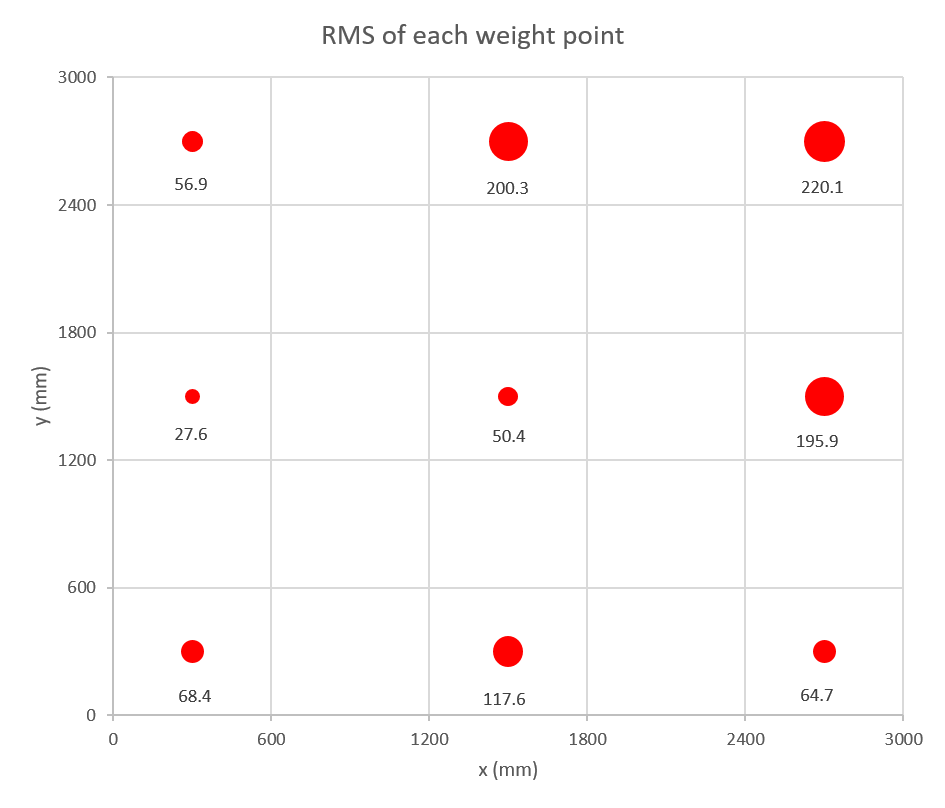
\includegraphics[height=!,width=\linewidth,keepaspectratio=true]
	{images/uwb_bench.png}
	\caption{以UWB定位之誤差量測實驗結果}
	\label{figure:localization_result}
\end{figure}

\paragraph{定位測試影片} 

本專題利用UWB之定位結果經過移動限制過濾器後繪製出行進軌跡,測試影片連結如下:

\begin{itemize}

\item
載具利用遙控行進場地一圈並繪製出軌跡圖
\url{<Put URL Here>}

\item
避障實驗一(靜態障礙物): 
\url{https://youtu.be/ve4Mln4D1xo}

\end{itemize}


\subsection{影像辨識}

...

\begin{figure}[h] % h means put this image here
\includegraphics[width=\columnwidth]{images/ground-vehicle.png}
\centering
\caption{地面無人載具實際場域驗證}
 \label{figure:ground-vehicle}
\end{figure}

\subsection{水面無人載具與RobotX競賽(進行中)}

本計畫已將所開發之演算法用於大型水面無人載具,Marine Advanced Research 所提供的自適應性波浪快艇 (Wave Adaptive Modular Vessel, WAM-V),並透過設計此船隻的感測、計算、及動力完成競賽任務。本論文使用之自適應性波浪快艇系統架構圖如圖~\ref{figure:system_diagram}所示,其中主要分成三個部分: 硬體、電路、軟體,分別在模擬與實際竹湖場域測試。

\begin{figure}[bht]
	\centering
	\includegraphics[height=!,width=\linewidth,keepaspectratio=true]
	{images/hardware_setting.png}
	\caption{本計畫將所開發的演算法移植到大型水上無人載具,將於2018年12月代表台灣第一次參與在夏威夷舉行的RobotX競賽。}
	\label{figure:system_diagram}
\end{figure}


